\documentclass[tikz,convert={outext=.png}]{standalone}
\begin{document}
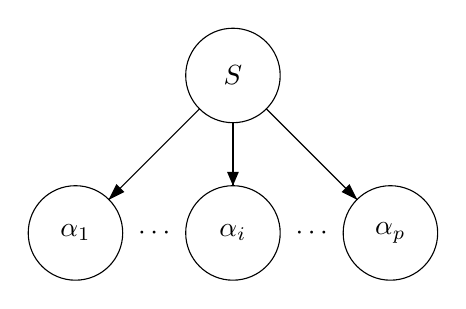
\begin{tikzpicture}[scale=0.2]
\tikzstyle{every node}+=[inner sep=0pt]
\draw [black] (0,0) circle (3);
\draw (0,0) node {$S$};

\draw [black] (-2.1, -2.1) -- (-7.9, -7.9);
\fill [black] (-7.9, -7.9) -- (-6.9, -7.4) -- (-7.4, -6.9);
\draw [black] (-10, -10) circle (3);
\draw (-10, -10) node {$\alpha_1$};

\draw (-5, -10) node {$\cdots$};

\draw [black] (0, -3) -- (0, -7);
\fill [black] (0, -7) -- (-.375, -6.125) -- (+.375, -6.125);
\draw [black] (0, -10) circle (3);
\draw (0, -10) node {$\alpha_i$};

\draw (+5, -10) node {$\cdots$};

\draw [black] (+2.1, -2.1) -- (+7.9, -7.9);
\fill [black] (+7.9, -7.9) -- (+6.9, -7.4) -- (+7.4, -6.9);
\draw [black] (+10, -10) circle (3);
\draw (+10, -10) node {$\alpha_p$};
\end{tikzpicture}
\end{document}
